\documentclass{beamer}

\usepackage{tikz}
\usetikzlibrary{graphs, decorations.pathmorphing}

\title{Optimizing Causal Reasoning in Concurrent Systems}
\author{Mahyar Karimi}

\begin{document}

\frame{\maketitle}

\begin{frame}
\frametitle{Optimizing with Minimal Enabling (1/3)}

Assume our effect $Y$ is a set of configuration vertices:
\[ Y = \{ \Pi_1, \cdots, \Pi_k \} \]

A cause of form $X = C_{i, j}$ filters out many vertices of the causal model
(assuming $|Y| = 1$).

\textbf{Question:} What about $X = M_{ \{i\}, j }$?
\end{frame}

\begin{frame}
\frametitle{Optimizing with Minimal Enabling (2/3)}

\begin{figure}
\centering
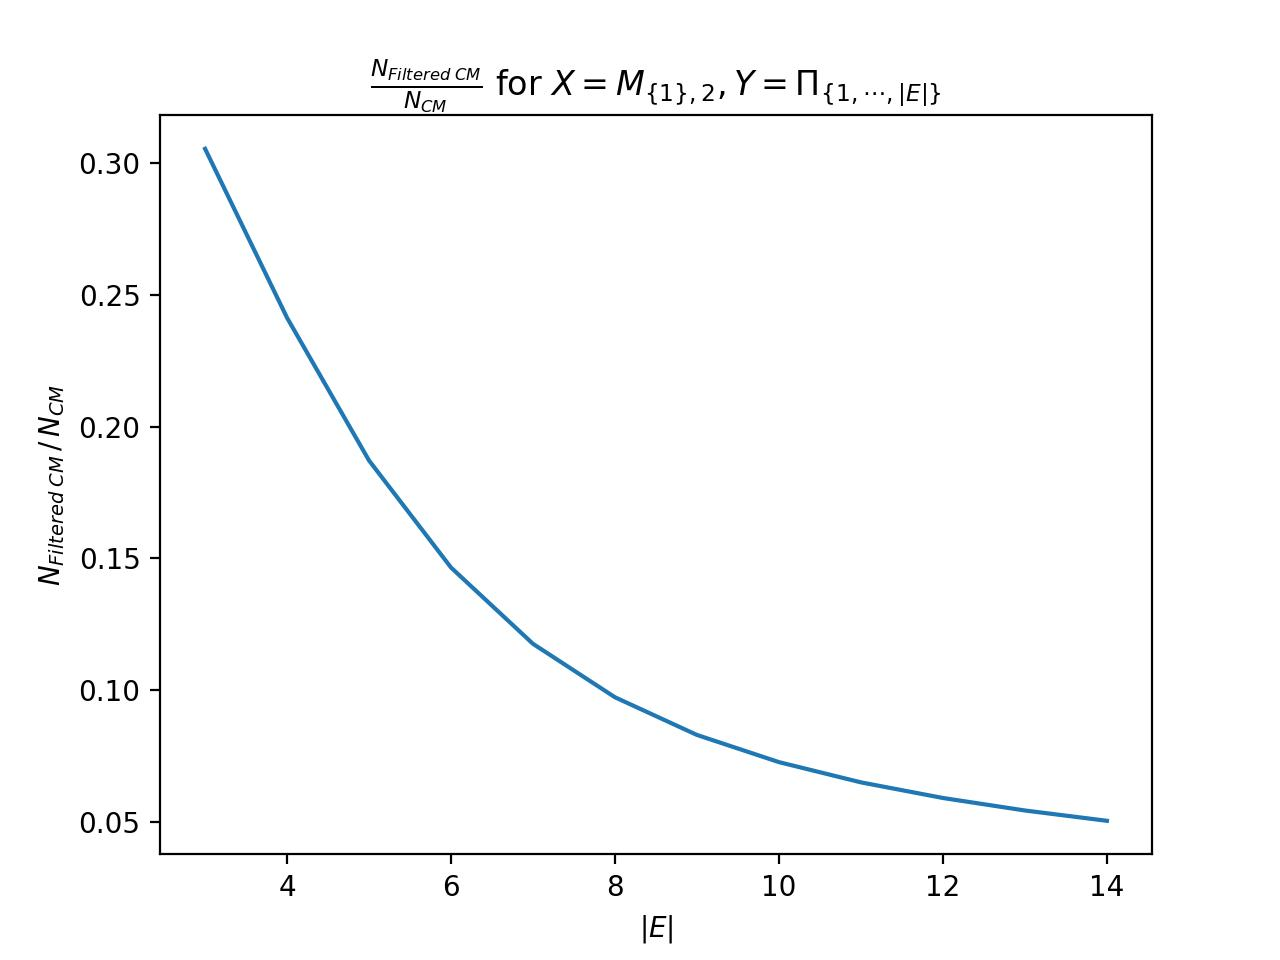
\includegraphics[scale=0.5]{plt/plt_m12_pi_all.jpg}
\end{figure}
\end{frame}

\begin{frame}
\frametitle{Optimizing with Minimal Enabling (3/3)}

\begin{figure}
\centering
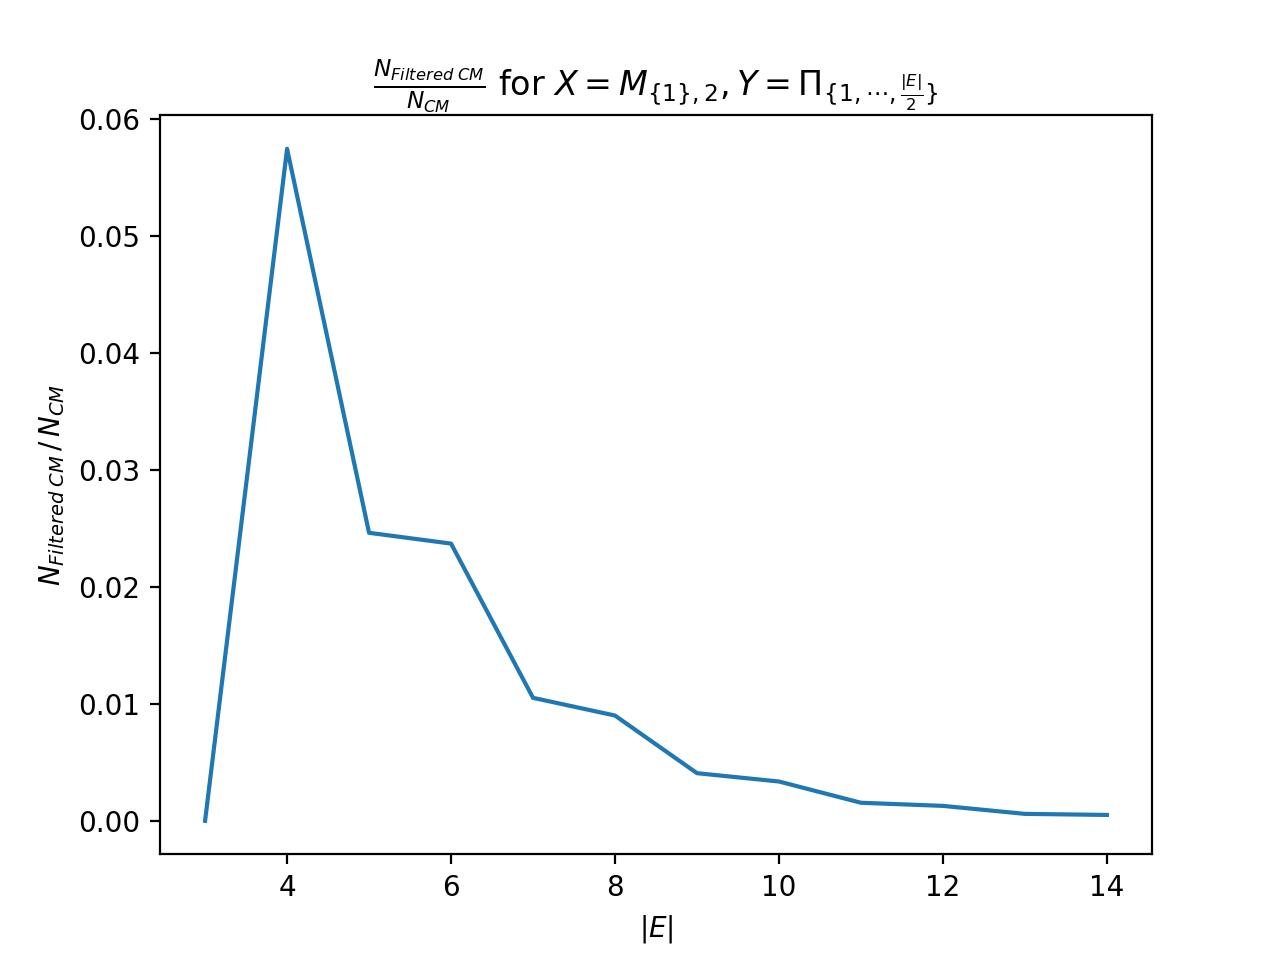
\includegraphics[scale=0.5]{plt/plt_m12_pi_half.jpg}
\end{figure}
\end{frame}

\begin{frame}
\frametitle{Min. En. Filtering: an Example (1/3)}

A sample network:

\begin{center}
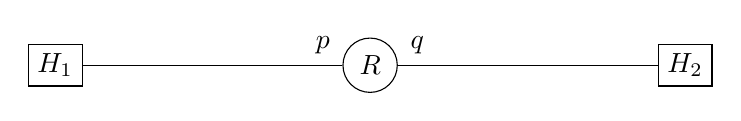
\begin{tikzpicture}
  \node[rectangle,draw] (H1) at (-4, 0) {$H_1$};
  \node[rectangle,draw] (H2) at (4, 0) {$H_2$};
  \node[circle,draw] (R) at (0, 0) {$R$};
  \node (p) at (-0.6, 0.25) {$p$};
  \node (q) at (0.6, 0.25) {$q$};
  \draw[-] (H1) -- (R);
  \draw[-] (R) -- (H2);
\end{tikzpicture}
\end{center}

Two messages are sent concurrently:

\begin{itemize}
  \item $f$: Forwards from $p$ to $q$ ($p \rightarrow q$)
  \item $t$: Drops every packet with tag $t$
\end{itemize}

\end{frame}

\begin{frame}
\frametitle{Min. En. Filtering: an Example (2/3)}
Configuration lattice for this network:

\begin{center}
\begin{tikzpicture}
  \node (null) at (0, 0) {$\varnothing$};
  \node (f) at (-1, -1) {$\{f_1\}$};
  \node (f-pq) at (-1, -2) {$\{ f_1, (p \rightarrow q)_2 \}$};
  \node[red] (f-pq-t) at (-1, -3) {$\{ f_1, (p \rightarrow q)_2, t_3 \}$};
  \node (f-t) at (-4, -2) {$\{ f_1, t_2 \}$};
  \node (t) at (4, -1) {$\{t_1\}$};
  \node (t-f) at (4, -2) {$\{t_1, f_2\}$};

  \draw[->] (null) -- (t);
  \draw[->] (null) -- (f);
  \draw[->] (t) -- (t-f);
  \draw[->] (f) -- (f-t);
  \draw[->] (f) -- (f-pq);
  \draw[->] (f-pq) -- (f-pq-t);
\end{tikzpicture}

\end{center}

Cause: $\{ f_1 \} \vdash (p \rightarrow q)_2$

Effect: $\{ f_1, (p \rightarrow q)_2, t_3 \}$ is a configuration

\textbf{Question:} How to show this cause?

\end{frame}

\begin{frame}
\frametitle{Min. En. Filtering: an Example (3/3)}

Adding new \textit{reason} vertices:

\begin{center}
\begin{tikzpicture}
  \node (null) at (0, 0) {$\varnothing$};
  \node (f) at (-1, -1) {$\{f_1\}$};
  \node[circle,draw,red] (reason) at (-1, -2) {};
  \node (f-pq) at (-1, -3) {$\{ f_1, (p \rightarrow q)_2 \}$};
  \node[red] (f-pq-t) at (-1, -4) {$\{ f_1, (p \rightarrow q)_2, t_3 \}$};
  \node (f-t) at (-4, -2) {$\{ f_1, t_2 \}$};
  \node (t) at (4, -1) {$\{t_1\}$};
  \node (t-f) at (4, -2) {$\{t_1, f_2\}$};
  \node[red] (m) at (1, -2) {$ \{f_1\} \vdash (p \rightarrow q)_2$};

  \draw[->] (null) -- (t);
  \draw[->] (null) -- (f);
  \draw[->] (t) -- (t-f);
  \draw[->] (f) -- (f-t);
  \draw[->,red] (f) -- (reason);
  \draw[->,red] (reason) -- (f-pq);
  \draw[->] (f-pq) -- (f-pq-t);
  \draw[->,red] (m) -- (reason);
\end{tikzpicture}
\end{center}

\end{frame}

\begin{frame}
\frametitle{Lattice-Based Causality}

Using the ``improved'' lattice to check causality:
\begin{itemize}
  \item Very straight-forward when the underlying lattice is a tree
\end{itemize}

\begin{center}
\begin{tikzpicture}
  \node[rectangle,draw] (m) at (-2, 0) {$s \vdash e$};
  \node[circle,draw] (reason) at (0, 0) {};
  \node[circle,draw] (effect) at (0, -3) {$Y$};
  \node (dots) at (1, -1) {$\ddots$};
  \node[circle,red,draw] at (2, -2) {$Y'$};
  \draw[->] (m) -- (reason);
  \draw[->,decorate,decoration=snake] (reason) -- (effect);
\end{tikzpicture}
\end{center}

For a generic improved lattice, the problem has more challenges.

\end{frame}
\end{document}